\documentclass[12pt]{ifi_thesis}
\setcounter{secnumdepth}{3} % Number \subsubsection
\setcounter{tocdepth}{3} % Include \subsubsection in ToC

\usepackage{tabularx} %tables
\usepackage{booktabs} %tables
\usepackage{rotating}
\usepackage[verbose]{placeins}
\usepackage{blindtext}
\usepackage{siunitx}
\usepackage[export]{adjustbox}
\usepackage{pdfpages}
\usepackage[hyphens]{url}
\usepackage{lipsum}
\usepackage{graphicx}
\usepackage{todonotes}
\usepackage[hidelinks]{hyperref} %HYPERLINK THE LINKS. DELETE FOR PRINT**
\usepackage{acro}
\acsetup{first-style=short, hyperref = true } %REMOVE hyperref for print
\usepackage{tabu}
\usepackage[utf8]{inputenc}
\usepackage[T1]{fontenc}
\usepackage{newtxtext,newtxmath}
\usepackage{soul} %for highlighting text usage: hl{}
\graphicspath{{Images/}}
%\renewcommand{\sfdefault}{phv}
%\renewcommand{\familydefault}{\sfdefault}
\renewcommand{\baselinestretch}{2}
% Must use biblatex to produce the Published Contents and Contributions.
\usepackage[
    backend=biber,natbib,
    % IMPORTANT: load a style suitable for your discipline
    style=authoryear
]{biblatex}
\renewcommand{\chaptername}{} % removes "chapter" word from table of contents
\usepackage{filecontents}
\usepackage{cleveref}
\newcommand\myshade{85}
\colorlet{mylinkcolor}{violet}
\colorlet{mycitecolor}{orange}
\colorlet{myurlcolor}{cyan}
\hypersetup{
  linkcolor  = mylinkcolor!\myshade!black,
  citecolor  = mycitecolor!\myshade!black,
  urlcolor   = myurlcolor!\myshade!black,
  colorlinks = true,
}


%%%%%%%%%%%%%%%%%%%%%%%%%%%%%%%%%%%%%%%%%%%%%%%%%%%%%%%%%%%%%%%%%%%%%%%%%%%%%%
%Code highlighting
%New colors defined below
\usepackage{listings} % for code display and highlighting

\definecolor{codegreen}{rgb}{0,0.6,0}
\definecolor{codegray}{rgb}{0.5,0.5,0.5}
\definecolor{codepurple}{rgb}{0.58,0,0.82}
\definecolor{backcolour}{rgb}{0.95,0.95,0.92}

\lstdefinestyle{mystyle}{
  backgroundcolor=\color{backcolour},   commentstyle=\color{codegreen},
  keywordstyle=\color{magenta},
  numberstyle=\tiny\color{codegray},
  stringstyle=\color{codepurple},
  basicstyle=\footnotesize,
  breakatwhitespace=false,         
  breaklines=true,                 
  captionpos=b,                    
  keepspaces=true,                 
  numbers=left,                    
  numbersep=5pt,                  
  showspaces=false,                
  showstringspaces=false,
  showtabs=false,                  
  tabsize=2
}
%"mystyle" code listing set
\lstset{style=mystyle}
%%%%%%%%%%%%%%%%%%%%%%%%%%%%%%%%%%%%%%%%%%%%%%%%%%%%%%%%%%%%%%%%%%%%%%%%%%%%%%



%abbreviations:
\DeclareAcronym{ami}{short=AMI,long=Advanced Metering Infrastructure}
\DeclareAcronym{pii}{short=PII,long=Personally identifiable information}
\DeclareAcronym{nve}{short=NVE,long=The Norwegian Water Resources and Energy Directorate}

\DeclareAcronym{ny}{short = NY ,long  = New York}
\DeclareAcronym{la}{short = LA ,  long  = Los Angeles}
\DeclareAcronym{un}{short = UN,long  = United Nations}
\DeclareAcronym{us}{short=USA,long=United states}

\nomenclature{GSD}{Global software development}

% Name of your .bib file(s)
\addbibresource{references.bib}
\addbibresource{references_Mendeley.bib}

\begin{document}

\title{To Slack or not to Slack; challenges of communication and coordination in distributed software development}
%Communication and coordination in distributed software teams\\in large-scale distributed %software development}
\author{Mehdi Noroozi}
\degreeaward{Master of Science in Informatics: Programming and Networks}
\university{University of Oslo}    
\address{Department of Informatics}                     
\unilogo{uio.png}                               
\copyyear{2018}  
\defenddate{}          
\orcid{}
\pagenumbering{gobble} %removes page number from the first pages
\rightsstatement{This work is licensed under a \href{https://creativecommons.org/licenses/by/4.0/}{Creative Commons Attribution 4.0 International License.}
\begin{figure}[hbt!]
\centering

\includegraphics[width=.2\textwidth]{cc.png}
\end{figure}}


\maketitle[logo]

\frontmatter
\begin{acknowledgements}
Typically the structure moves from thanking the most formal support to the least formal thanks as detailed above–funders, supervisors, other academics, colleagues, and finally family. This makes sense according to the logic of incremental progression because the informal thanks to family are often the most heartfelt. Close family members are often the people who gave the most (although some supervisors are likely to feel this is not true).

It is important that a student acknowledges the formal carefully, though: any person or institution that has contributed funding to the project, other researchers who have been involved in the research, institutions that have aided the research in some way. They should also acknowledge proofreaders and editors. Such formal thanks are usually in the first paragraph or two.
\end{acknowledgements}
\begin{abstract}


Globalization is affecting our daily life more and more every day. In addition to affecting every and each person, it is also affecting businesses around the globe and to cope with it managers and other decision-makers should think of new and innovative ways to keep their businesses going on. Software development industry is also no exception and was one of the industries that since the 1990s started to merge in the global market. The expansion of access to the internet around the world has evaded the need for co-located software teams and has made it possible to freely collaborate and work on software projects from all around the world. \\

There are several success stories regarding the distributed and global software development, however, it is not free from mistakes and huge financial losses. Among the several issues that distributed software development is facing, communication and coordination are named in several studies as the prominent cause of failure in distributed projects. In the absence of face-to-face communication which is considered to be the richest form of communication and the presence of cultural and language barriers, misunderstanding is unavoidable and problems can easily escalate.\\

In this thesis, we are going to take a closer look at communication and coordination issues in distributed software teams through analyzing Slack chat logs of two distributed teams as well as running a survey among software developers. In the end, we are going to give some suggestions for improvement of communication and coordination in distributed teams.\\

The results gained through the analysis of Slack chat logs and results of the survey are in agreement with several other studies and research done on the topic. 


\end{abstract}
\tableofcontents
\listoffigures
\listoftables
\printnomenclature
\printacronyms

\mainmatter
%\chapter{Example}


Start off all chapters with \verb|chapter|. \index{chapter!numbered} \verb|\extrachapter| will give you an unnumbered chapter that's added to the Table of Contents. \index{chapter!unnumbered}


If you're new to \LaTeX{} and would like to begin by learning the basics, please see our free online course available at:\\ \url{https://www.overleaf.com/latex/learn/free-online-introduction-to-latex-part-1} \index{LaTeX@\LaTeX}


\section{This is a Section}

\begin{figure}[hbt!]
\centering

\includegraphics[width=.3\textwidth]{uio.png}
\caption{This is a figure}\label{fig:logo}
\index{figures}
\end{figure}

\subsection{This is a subsection}

\begin{table}[hbt!]
\centering
\begin{tabular}{ll}
\hline
Area & Count\\
\hline
North & 100\\
South & 200\\
East & 80\\
West & 140\\
\hline
\end{tabular}
\caption{This is a table}
\label{tab:sample}
\index{tables}
\end{table}


Here's an endnote.\endnote{Endnotes are notes that you can use to explain text in a document.}

\section{This is code Section}

\begin{lstlisting}[language=Python, caption=JSON example]
 {
     "type": "message",
     "user": "U3MPT6W77",
     "text": "I don't understand the question :slightly_smiling_face:",
     "ts": "1495181765.592074"
  },
\end{lstlisting}

\part{Introduction}
\chapter{Introduction}
%%%%%%%%%%%%%%%%%%%%%%%%%%%%%%%%%%%%%%%%%%%%%%%%%%%%%%%%%%%%%%%%%%%%%%%%%%%%%%%%%%%%%%

\section{Motivation and background}
%%%%%%%%%%%%%%%%%%%%%%%%%%%%%%%%%%%%%%%%%%%%%%%%%%%%%%%%%%%%%%%%%%%%%%%%%%%%%%%%%%%%%%

\section{Research objective}
%%%%%%%%%%%%%%%%%%%%%%%%%%%%%%%%%%%%%%%%%%%%%%%%%%%%%%%%%%%%%%%%%%%%%%%%%%%%%%%%%%%%%%

\section{Thesis Structure}
%%%%%%%%%%%%%%%%%%%%%%%%%%%%%%%%%%%%%%%%%%%%%%%%%%%%%%%%%%%%%%%%%%%%%%%%%%%%%%%%%%%%%%





Distributed Software Development (DSD) is today practiced commonly in the software industry in both large and small companies and organizations \citep{shrivastava2010distributed}. This means that software development teams are not physically sitting in the same place and hence don’t have the opportunity to meet or speak to other team members in person regularly \citep{layman2006essential}. This distribution might mean sitting in two different buildings or sitting on two different continents. Global Software Development (GSD) is a special form of DSD in which the distribution of teams are across national borderlines \citep{sahay2003global}. 

Communication has an important role in the success of GSD \citep{carmel2001tactical,french1998study}, especially informal communication \citep{herbsleb2003empirical}. The processes of communication, coordination, and collaboration are of the utmost importance and key aspects of the software development process \citep{colomo2014agile}. Research shows that distance has a big impact on the performance of projects \citep{damian2003global,herbsleb2001global}. Communication is also an important part of all software development practices \citep{layman2006essential}. Empirical research also shows that developers are in need of ad hoc and informal communication \citep{grinter1998recomposition,kraut1995coordination}. Therefore any shortcomings in communication between the teams and team members will heavily impact the success of GSD projects \citep{layman2006essential}.

Face-to-face meetings are the most efficient and ideal type of communication, but in GSD which teams are spread in different places, often with time zone differences, this is not possible and therefore might be challenging to achieve effective communication between teams and team members. In the presence of temporal distance between the teams and team members real-time and synchronous communication using a phone, and text or video chat is difficult to achieve \citep{holmstrom2006agile,kommeren2007philips}.

Casey and Richardson have worked on a case in which two virtual teams located in Ireland and Malaysia used just an asynchronous type of communication, e-mail \citep{casey2008impact}. Using asynchronous communication tools, like e-mail increases the chances of misunderstanding and ambiguity of information. Also, the communication is not really effective if the parties communicating with each other don’t understand each other \citep{kommeren2007philips,cataldo2007coordination}.

Receiving delayed feedback is also another challenge faced by remotely located teams, which itself is again a side effect of asynchronous communication \citep{conchuir2006exploring,holmstrom2006agile}. Research shows that using asynchronous communication tools in remote teams increases dramatically the time it takes to receive a response \citep{holmstrom2006global}. It is also true that a software engineer usually spends most of her time in searching and exchanging information, rather than doing anything else, and as a result, this can lead to delays in completing the project and increases the cost of the project. One of the ways to mitigate this problem is through proper project coordination \citep{dumitriu2006issues}. \hl{why synchronous is important (last 2 paragraphs are about it)}

\part{Background}
\chapter{Communication}
%%%%%%%%%%%%%%%%%%%%%%%%%%%%%%%%%%%%%%%%%%%%%%%%%%%%%%%%%%%%%%%%%%%%%%%%%%%%%%%%%%%%
Distributed software development (\ac{dsd}) is today practiced commonly in the software industry in both large and small companies and organizations \citep{shrivastava2010distributed}. This means that software development teams are not physically sitting in the same place and hence don’t have the opportunity to meet or speak to other team members in person regularly \citep{layman2006essential}. This distribution might mean sitting in two different buildings or sitting on two different continents.Global Software Development \ac{gsd} is a particular form of \ac{dsd} in which the distribution of teams are across national borderlines \citep{sahay2003global}. 

All team members in both collocated and distributed software teams communicate with each other using some form of Internet-based communication tool \citep{Kirkman2005}. Communication has an important role in the success of \ac{gsd} \citep{carmel2001tactical,french1998study}, especially informal communication \citep{herbsleb2003empirical}. The processes of communication, coordination, and collaboration are of the utmost importance and key aspects of the software development process \citep{colomo2014agile}. Using internet-based communication in teams have several benefits for companies, such as easier access to the global market, preserving the environment, and having team members in different locations around the globe that will enable the companies to work non-stop \citep{Cascio2000}. Research also shows that distributed teams, that are inevitably using internet-based communication, performing better than traditional teams in tasks like brainstorming because of the elimination of production blocking effects \citep{Espinosa2015}.

However, there are some challenges that threats distributed teams. High pressure in mastering advanced communication technology and lack of nonverbal communication, as well as problems in forming trust are some of them \citep{Jarvenpaa1998,Kayworth2002}. Misunderstanding might also happen easily in the absence of sentiment and meta-level information, such as body language \citep{Cramton2001}. Also, the type of communication technology and tools will affect the communication in teams and might lead to limited information sharing between distributed team members \citep{Gilson2015}.

Research shows that distance has a significant impact on the performance of projects \citep{damian2003global,Herbsleb2001a}. Communication is also an essential part of all software development practices \citep{layman2006essential}. Empirical research also shows that developers are in need of ad hoc and informal communication \citep{grinter1998recomposition,kraut1995coordination}. Therefore any shortcomings in communication between the teams and team members will profoundly impact the success of \ac{gsd} projects \citep{layman2006essential}.

Face-to-face meetings are the most efficient and ideal type of communication \citep{Kirkman2004}, but in \ac{gsd} which teams are spread in different places, often with time zone differences, this is not possible and therefore might be challenging to achieve effective communication between teams and team members. In the presence of temporal distance between the teams and team members, real-time and synchronous communication by using a phone, text or video chat is challenging to achieve \citep{holmstrom2006agile,kommeren2007philips}.

\citet{casey2008impact} have worked on a case in which two distributed teams located in Ireland and Malaysia used just an asynchronous type of communication, e-mail. In that case, using asynchronous communication tools, like e-mail increased the chances of misunderstanding and ambiguity of information. Also, the communication is not adequate if the parties communicating with each other don’t understand each other \citep{kommeren2007philips,cataldo2007coordination}.

Receiving delayed feedback is also another challenge faced by remotely located teams, which itself is again a side effect of asynchronous communication \citep{conchuir2006exploring,holmstrom2006agile}. Research shows that using asynchronous communication tools in remote teams increases dramatically the time it takes to receive a response \citep{holmstrom2006global}. 

It is also true that a software engineer usually spends most of her time in searching and exchanging information, rather than doing anything else, and as a result, this can lead to delays in completing the project and increases the cost of the project. One of the ways to mitigate this problem is through proper project coordination \citep{dumitriu2006issues}. 

%%%%%\hl{why synchronous is essential (last 2 paragraphs are about it)}

%%%%%%%%%%%%%%%%%%%%%%%%%%%%%%%%%%%%%%%%%%%%%%%%%%%%%%%%%%%%%%%%%%%%%%%%%%%%%%%%%%%%%%%%%%%%%%%%%%
\section{Media Richness and Media Synchronicity Theories}
%%%%%%%%%%%%%%%%%%%%%%%%%%%%%%%%%%%%%%%%%%%%%%%%%%%%%%%%%%%%%%%%%%%%%%%%%%%%%%%%%%%%%%%%%%%%%%%%%%

Seminal media theory tries to categorize the communication media based on their effectiveness and "richness" to express the link between communication and technology, and in this regard sees the richest medium in face-to-face encounters that is able of carrying all the verbal and non-verbal messages and minimizes the ambiguity, and sees the written mediums, such as email, as the least rich medium of communication \citep{Daft1986,Hassell2016}.

Later, \citet{Dennis2008} proposed the Media synchronicity theory to address the limitations and shortcomings of the other media theory proposed before. Media synchronicity theory discusses the different attributes of several types of media and attempts to look at them more precisely.

\citet{Dennis2008} suggest five attributes:

1- Regardless of the medium to be synchronous or asynchronous, immediate feedback is present.\\
2- Availability and diversity of symbols.\\
3- Availability of the ability to have several parallel conversations at the same time.\\
4- The messages can be rehearsed before transmission.\\
5- The conversations and messages sent and received can be retrieved.\\


\begin{figure}[hbt!]
\centering
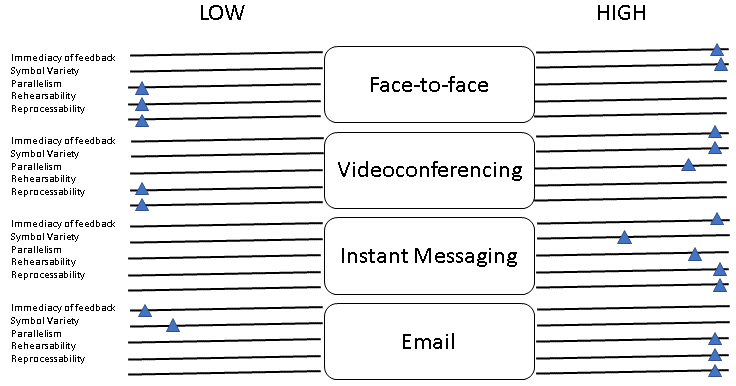
\includegraphics[width=.99\textwidth]{maruping.png}
\caption{Breakdown of communication media based on the criteria proposed by the media synchronicity theory inspired by \citet{Maruping2004}}\label{fig:maruping}
\index{figures}
\end{figure}

%%%%%%%%%%%%%%%%%%%%%%%%%%%%%%%%%%%%%%%%%%%%%%%%%%%%%%%%%%%%%%%%%%%%%%%%%%%%%%%%%%%%%%%%%%%%%%%%%%
\section{Enterprise Social Networks}
%%%%%%%%%%%%%%%%%%%%%%%%%%%%%%%%%%%%%%%%%%%%%%%%%%%%%%%%%%%%%%%%%%%%%%%%%%%%%%%%%%%%%%%%%%%%%%%%%%

Because of the value that organizations see in using social media at the workplace and high demand for such platforms, during the recent years several companies have started to develop tools such as Slack, HipChat, Yammer, and Workplace by Facebook \citep{Leroy2013}. These applications are known as Social Networking Platforms (\ac{snp}) or Team Communication Platforms (\ac{tcp}), and can be categorized under communication methods that are called Enterprise Social Networking (\ac{esn}) or Enterprise Social Media (\ac{esm}).

One thing that differentiates usual social media such as Facebook and Twitter from \ac{esn} is that social media is open to public and everyone can use them but access to ESN is limited to employees and those with whom the company needs to get in touch regularly \citep{Turban2011}.

\citet{Leonardi2013} describe four attributes which a platform should provide for its users to be considered as an \ac{esn}:\\
1- The users must be able to send and receive messages to individual members as well as the whole or a group of members. \\
2- Either explicitly or implicitly should be able to choose and show special coworkers as their communication partners.\\
3- It must be possible to share files with other users.\\
4- At any time it must be possible for any user to view all the conversations that are done publicly, consisting of text messages and file shared.

\ac{esn} acts as a forum for its members where they are able to communicate with other co-workers in the same organization \citep{Leonardi2014} in which business goals, such as enhanced knowledge sharing, easier access to expertise, and innovation can be reached better in a more secure and private environment \citep{Leonardi2013}.

If the \ac{esn} is correctly managed it can boost the productivity and motivation of employees, enhance collaboration between the different actors in the organization, and lead to more learning for team members \citep{Leon2017}. It also enables people in different locations to be able to communicate and become more involved in innovation, revenue creation, and socio-economic growth \citep{Qi2016}.

One of the problems that can be associated with the long-term use of \ac{esn}s is that employees might feel isolated because of limited face-to-face encounters with other people \citep{Kane2014}, but at the same time \ac{esn} is not designed and meant to completely replace personal and physical encounters \citep{Zhang2013a}.

Also because of the learning curve associated with any new tool, organizations might have not completely reached their goals in increasing collaboration between their employees \citep{Anderson2016}. However, developing an open culture among the employees and using an \ac{esn} which have similarities to social media that employees use in their private life may help to improve the usage of \ac{esn} by employees \citep{Korzynski2014}. 


%%%%%%%%%%%%%%%%%%%%%%%%%%%%%%%%%%%%%%%%%%%%%%%%%%%%%%%%%%%%%%%%%%%%%%%%%%%%%%%%%%%%%%%%%%%%%%%%%%
%%%%%%%%%%%%%%%%%%%%%%%%%%%%%%%%%%%%%%%%%%%%%%%%%%%%%%%%%%%%%%%%%%%%%%%%%%%%%%%%%%%%%%%%%%%%%%%%%%
\chapter{Coordination} \label{coordinering}
%%%%%%%%%%%%%%%%%%%%%%%%%%%%%%%%%%%%%%%%%%%%%%%%%%%%%%%%%%%%%%%%%%%%%%%%%%%%%%%%%%%%%%%%%%%%%%%%%%
%%%%%%%%%%%%%%%%%%%%%%%%%%%%%%%%%%%%%%%%%%%%%%%%%%%%%%%%%%%%%%%%%%%%%%%%%%%%%%%%%%%%%%%%%%%%%%%%%%

Scholars have defined coordination in different ways. \citet{Malone1988} defines coordination as for when several actors seek goals together and must do things to organize themselves in order to reach that goal while a single actor seeking the same goals does not have to do the same things. He calls these extra activities needed for organizing, coordination. Later, \citet{Malone1994} adjusted the definition of coordination to managing of dependencies. The definition is justified in that there are interdependent associations between activities, and contrive with these relations effectively, coordination mechanisms are needed \citep{Deng2007}.

Coordination from Osifo's (2012) point of view can be classified as part of an organization. At the same time, \citep{Beuselinck2007} and \citep{Osifo2012} confirm Malone and Crowston’s (\citeyear{Malone1988}) definition which states that there would be no need for coordination if there is no dependency and relation.

There are two aspects of the coordination which are important for organizations, internal and external coordination. Internal coordination is important to achieve cooperation by having support and clarity. Without internal coordination, it would be difficult to achieve satisfactory progress in the projects. It also provides help in setting rules and criteria. External coordination also plays an important role in setting limits so that the project always stays in focus and continues on the right path \citep{Osifo2012}.

Coordination is part of nearly every single part of a project and is rarely employed alone by only one coordination mechanism \citep{Osifo2012}. Almost always coordination of a particular project or organization is accomplished by using several coordination mechanisms \citep{Dietrich2013}.

%%%%%%%%%%%%%%%%%%%%%%%%%%%%%%%%%%%%%%%%%%%%%%%%%%%%%%%%%%%%%%%%%%%%%%%%%%%%%%%%%%%%%%%%%%%%%%%%%%
\section{Van de Ven model of coordination}
%%%%%%%%%%%%%%%%%%%%%%%%%%%%%%%%%%%%%%%%%%%%%%%%%%%%%%%%%%%%%%%%%%%%%%%%%%%%%%%%%%%%%%%%%%%%%%%%%%

Researchers have suggested several coordination mechanisms. \citet{Strode2012} states that synchronization, structure, and boundary spanning are mechanisms which are worthy for efficient coordination. \citet{Mintzberg1980} believes that mechanisms such as mutual adjustment, direct supervision, and standardization are of importance in coordination.

\citet{VanDeVen1976} suggest another coordination model which is somehow similar to other scholars but adds the notion of team to the coordination strategy. For example, they believe that mutual adjustment in co-located teams is reached by mutual interactions.

\citet{VanDeVen1976} suggest another coordination model which is somehow similar to the models suggested by other scholars but adds the notion of team to the coordination strategy. For example, they believe that mutual adjustment in co-located teams is reached by mutual interactions.
Still, in the case of the ways in which coordination can be achieved it is somewhat similar to the theory suggested by  \citet{Thompson2014}. According to \citet{VanDeVen1976}, there are three modes for coordination of work activities; impersonal, personal, and group mode of coordination.

In Van de Van's model, the focus is on the team and how based on the change of some factors the coordination modes changes. \citet{VanDeVen1976} suggest that coordination mechanisms in every one of those three modes are utilized in different combinations to reach a certain collective goal.

%%%%%%%%%%%%%%%%%%%%%%%%%%%%%%%%%%%%%%%%%%%%%%%%%%%%%%%%%%%%%%%%%%%%%%%%%%%%%%%%%%%%%%%%%%%%%%%%%%
\section{Impersonal mode of coordination}
%%%%%%%%%%%%%%%%%%%%%%%%%%%%%%%%%%%%%%%%%%%%%%%%%%%%%%%%%%%%%%%%%%%%%%%%%%%%%%%%%%%%%%%%%%%%%%%%%%

Anything that needs the minimum amount of verbal communication between actors once implemented and in nature is relevant to programming, technical means, and administrative coordination can be correlated with impersonal mode of coordination \citep{Boos2011,VanDeVen1976}.

\citet{Kraut1995a} suggest some coordination techniques that can reduce some of the coordination challenges when a mixture of large size, intricacy, and interdependence occurs simultaneously;  using technical tools, modularization, and formal procedures are some of the suggested techniques.

Keeping large-scale projects coordinated by using tools and having a shared system to keep the record of documents is of utmost importance. Some of the examples of impersonal coordination mechanisms found in large-scale agile are standardization of work process (such as following the scrum methodology), having rules for QA, and use of tools such as Jira \citep{Nyrud2017b}.

%%%%%%%%%%%%%%%%%%%%%%%%%%%%%%%%%%%%%%%%%%%%%%%%%%%%%%%%%%%%%%%%%%%%%%%%%%%%%%%%%%%%%%%%%%%%%%%%%%
\section{Personal mode of coordination}
%%%%%%%%%%%%%%%%%%%%%%%%%%%%%%%%%%%%%%%%%%%%%%%%%%%%%%%%%%%%%%%%%%%%%%%%%%%%%%%%%%%%%%%%%%%%%%%%%%

In the personal mode, according to \citet{VanDeVen1976}, coordination happens through feedback or mutual adjustments on the input information that an actor receives from the other actors. Mutual task adjustments happen either through vertical or horizontal communication channels.
Line managers and unit supervisors are often the mechanisms of vertical communication which is hierarchical in nature \citep{Thompson2014}. But horizontal communication is more about individual people in teams that communicate on a one-to-one basis with other team members, and it is usually non-hierarchical \citep{VanDeVen1976}.

\citet{Mintzberg1980} divides coordination mechanisms to mutual adjustment and direct supervision. These two mechanisms are similar to vertical and horizontal channels of communication in the personal mode of coordination. Mutual adjustment happens when people in the team informally communicate with other teammates to coordinate their tasks. In the direct supervision, a person from a higher level than the others, like the head of a team, gives some instructions that must be followed by other team members who work under her supervision.


%%%%%%%%%%\hl{Hva er egentlig IM? A tool? Impersonal. Mutual adjustment -> vertical/horizontal personal mode? 1to1 group mode unscheduled? channels.}

Personal mode of coordination consists of both informal and formal communication \citep{Kraut1995a}. Also, it is more valuable in unscheduled and unexpected encounters \citep{Boos2011,Dickenson1997}. \citet{Kraut1995a} suggest that informal communication between team members while discussing work-related matters in front of water or coffee machine forms a large amount of coordination and that coordination does not only happen in formal meetings.

The success of coordination is dependent on some factors. Trust is one of those factors because organizational performance is realized by the network created by coordination \citep{DeJong2016}. Reduced coordination is in direct association with trust \citep{RoohullahJan2016}. And its importance is because it is the central part of decent coordination \citep{Osifo2012}. 

%%%%%%%%%%%%%%%%%%%%%%%%%%%%%%%%%%%%%%%%%%%%%%%%%%%%%%%%%%%%%%%%%%%%%%%%%%%%%%%%%%%%%%%%%%%%%%%%%%
\section{Group mode of coordination}
%%%%%%%%%%%%%%%%%%%%%%%%%%%%%%%%%%%%%%%%%%%%%%%%%%%%%%%%%%%%%%%%%%%%%%%%%%%%%%%%%%%%%%%%%%%%%%%%%%

Group mode of coordination, like the personal mode, happens by feedback and mutual adjustments but with the difference that all these happen in the group in unscheduled or scheduled meetings and consists of more planned communication \citep{VanDeVen1976}.

\citet{Dietrich2013} suggest three other coordination mechanisms that are important in large-scale projects. Those three mechanisms are called centralized, decentralized, and balanced patterns, which respectively are about coordination at the group level that is either scheduled or unscheduled, coordination between teammates which are not scheduled, and at last the combination of the first two ones.

The coordination strategy that \citet{Strode2012} have suggested involves three principal concepts of synchronization, structure, and boundary spanning that assist in managing dependencies. Regarding the group mode of coordination, synchronization has more relevance and importance and is gained within synchronization activities. These activities are done usually once at the beginning of the project, but also can happen several times during the project so that the team members are aware of the project requirements and maintain this understanding during the whole project \citep{Strode2012}.

%%%%%%%%%%%%%%%%%%%%%%%%%%%%%%%%%%%%%%%%%%%%%%%%%%%%%%%%%%%%%%%%%%%%%%%%%%%%%%%%%%%%%%%%%%%%%%%%%%
%%%%%%%%%%%%%%%%%%%%%%%%%%%%%%%%%%%%%%%%%%%%%%%%%%%%%%%%%%%%%%%%%%%%%%%%%%%%%%%%%%%%%%%%%%%%%%%%%%
\chapter{Distributed teams} \label{dt}
%%%%%%%%%%%%%%%%%%%%%%%%%%%%%%%%%%%%%%%%%%%%%%%%%%%%%%%%%%%%%%%%%%%%%%%%%%%%%%%%%%%%%%%%%%%%%%%%%%
%%%%%%%%%%%%%%%%%%%%%%%%%%%%%%%%%%%%%%%%%%%%%%%%%%%%%%%%%%%%%%%%%%%%%%%%%%%%%%%%%%%%%%%%%%%%%%%%%%

Distributed teams are called by several names, but it is generally agreed that a team is considered as distributed when its members are spread at least in two locations \citep{Hinds2005}. This physical separation can range between two different offices in the same city or country or people sitting in different countries and continents \citep{Mortensen2001}. Here I will now discuss some of the advantages and disadvantages of using distributed software teams.

%%%%%%%%%%%%%%%%%%%%%%%%%%%%%%%%%%%%%%%%%%%%%%%%%%%%%%%%%%%%%%%%%%%%%%%%%%%%%%%%%%%%%%%%%%%%%%%%%%
\section{Advantages of using distributed teams}
%%%%%%%%%%%%%%%%%%%%%%%%%%%%%%%%%%%%%%%%%%%%%%%%%%%%%%%%%%%%%%%%%%%%%%%%%%%%%%%%%%%%%%%%%%%%%%%%%%

When evaluating distributed teams and discussing the dynamic situation of global business it is essential to know the advantages that this type of team structure offers a company that uses it. 

1- Companies can benefit from a much more bigger pool of global experts in different subjects and recruit some of the best talents that might not be available locally or might be expensive to recruit \citep{Snyder2003}. Relocation is costly and stressful and today most of the workers try to avoid it \citep{Lipnack1997,Joinson2002}. Human resources of companies can be increased in this case, because especially skilled members of the company can serve on several teams simultaneously \citep{Hertel2004}. 

2- Costs associated with traveling and accommodation will be reduced drastically or completely eliminated. \citet{Baskerville2007} report that IBM by using distributed teams saved \$50 million in travel and downtime costs.

3- Distributed teams encourages multiculturalism and discourages discrimination by age and race because the members are evaluated by the performance and productivity. This type of team fosters equality and fairness among the employees \citep{Bergiel2007}.

4- Because of the diversity and heterogeneity of distributed teams, these teams are more effective and promote creativity among its members compared to more rigid structure of traditional teams which are limited by time and space \citep{Bergiel2008}.

%%%%%%%%%%%%%%%%%%%%%%%%%%%%%%%%%%%%%%%%%%%%%%%%%%%%%%%%%%%%%%%%%%%%%%%%%%%%%%%%%%%%%%%%%%%%%%%%%%
\section{Disadvantages of using distributed teams}
%%%%%%%%%%%%%%%%%%%%%%%%%%%%%%%%%%%%%%%%%%%%%%%%%%%%%%%%%%%%%%%%%%%%%%%%%%%%%%%%%%%%%%%%%%%%%%%%%%

1- Managing conflicts between team members in distributed teams is a big challenge \citep{Hinds2003}. Lack of good communication tools and a shared identity in distributed teams lead to conflict \citep{Hinds2005a}. 

2- Coordination and cohesion may be reduced in distributed teams which in turn affects work performance \citep{DeRosa2004}.

3- Feeling isolated and lack of face-to-face social interaction is also common in distributed teams that don't have the opportunity of meeting their colleagues as often as traditional teams \citep{Kiesler2002}.

%%%%%%%%%%%%%%%%%%%%%%%%%%%%%%%%%%%%%%%%%%%%%%%%%%%%%%%%%%%%%%%%%%%%%%%%%%%%%%%%%%%%%%%%%%%%%%%%%%
%%%%%%%%%%%%%%%%%%%%%%%%%%%%%%%%%%%%%%%%%%%%%%%%%%%%%%%%%%%%%%%%%%%%%%%%%%%%%%%%%%%%%%%%%%%%%%%%%%
\chapter{Slack} \label{slack}
%%%%%%%%%%%%%%%%%%%%%%%%%%%%%%%%%%%%%%%%%%%%%%%%%%%%%%%%%%%%%%%%%%%%%%%%%%%%%%%%%%%%%%%%%%%%%%%%%%
%%%%%%%%%%%%%%%%%%%%%%%%%%%%%%%%%%%%%%%%%%%%%%%%%%%%%%%%%%%%%%%%%%%%%%%%%%%%%%%%%%%%%%%%%%%%%%%%%%

Since analyzing Slack constitutes an important part of this thesis and Slack is more than yet another chat application I decided to give a description of this platform and some of its most important functions that makes Slack one of the most popular communication and collaboration systems used in software teams.

In order to describe Slack both secondary data obtained from its website, as well as my own experience as a lack user is used. The reader of this introduction will get a sense of what Slack, as a sophisticated enterprise social network is.

Slack was started in 2013 and has more than eight million active users every day, three million of which are paid users \citep{Lynley2018}. It has turned a contemporary form of communication, i.e texting, into a workplace app. Its valuation is \$ 5.1 billion. Although it has recently encountered by some big players in the market, like Microsoft, Google, and Facebook, still 43 percent of Fortune 100 companies are using Slack. Its popularity among startup companies is the same, if not more than the big enterprises \citep{Rodriguez2018}.

\citet{Williams2015a} who has created a document on how to use the Slack, says that Slack can be seen as a chat room where the whole company and its different teams can be broken into smaller channels for group discussion. Channels are often created to discuss a certain topic and are like the old chat rooms. Like any other communication platform, sending direct messages to individuals is also possible in Slack.

Slack is a multi-platform software, meaning that it can be used on all kinds of operating systems on all mobile phones, as well as desktops and laptops. The user can be notified of several things by several ways. Direct messages and mentions usually generate notifications that can both received by email, if the user is not online, or will be shown on the Slack app. These notifications are highly customizable and can be suppressed to avoid being overwhelmed by the number of notifications. 

Teams are another feature of Slack. Groups of people who are working together can use it to communicate with each other. It can be created simply by visiting Slack's website. A team must have an owner and can have several admins who will enforce the team rules. Often working in large organizations means being part of several Slack teams. There is also possible to work in several workspaces, as each one works as a separate team that is connected to the Slack's enterprise network.  All the teams and works places are available on the web, desktop, and mobile version of Slack.

Figure \ref{fig:slack} shows an screen shot of a Slack channel.
\begin{figure}[hbt!]
\centering
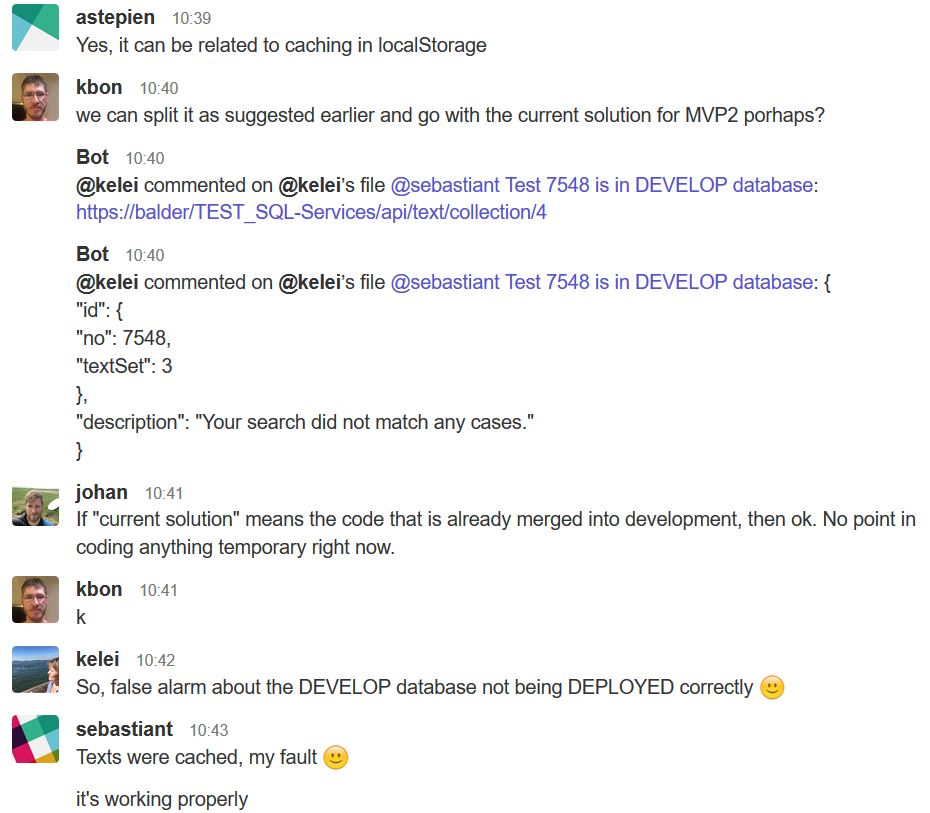
\includegraphics[width=\linewidth, frame]{slack.JPG}
\caption{A screenshot from Slack}\label{fig:slack}
\index{figures}
\end{figure}


Channels in Slack are used as chat rooms for group conversation. Different channels are usually created to discuss certain topics. These channels can either be public or private. Public channels are visible to the entire team and all the team members can join them. But private channels need an invitation to join and usually, admin of the channels adds the other users to the channel.
 
Everything shared on Slack, including text, image, file, and other types of posts can be searched by users. The information shared in private channels can just be searched and found by the members of the channel. Also paid customers of Slack have the ability to invite external users. In that case, only the information shared in the respective channels can be searched and found by the external member.

The other way that users can communicate in Slack is by direct messages (DM). It is possible to send a DM to up to eight other users simultaneously. Obviously, these messages can be just seen and searched by those who are involved in the messages. It is also possible to call up to fifteen users at the same time if the team is a using the paid service, but in the free version, just one-on-one calls are supported. 

Using emoji is another way of communicating in Slack, it can be both used by the user who is writing the message to communicate her emotions (Figure \ref{fig:slack}), as well as by the readers of the message who can "react" to the message and communicate their emotion with the sender of the message. it is also common to get the attention of someone or the whole members of a channel by putting @ before the username of the users. In this case, users will immediately get a notification if they are online, or will get an email in case they are offline.

Moreover, the notifications that the user receives can be heavily customized to meet the needs of the user. Users, for example, may define certain words and phrases that when appeared in chat messages visible by the user the system will generate a notification. Notification can be manipulated based on several properties, like time, date and location. For example, one can decide not to receive any notification during weekends. Another capability that Slack users have is the ability to organize messages by pinning them or starring them, in order to get access to important messages more easily late on. All the sent messages can also be edited after being sent. And the appearance of the Slack can be customized by changing themes and colors to match the taste of every individual user. 

One of the reasons that Slack is so popular in teams is because of its ability to integrate with lots of external services, like Google Calendar, GitHub, IFTTT, and many more \citep{Williams2015}. Users also have the possibility of sending and sharing files and folders. It is also possible for users to make voice and video calls. All the function mentioned in this section are provided free of charge but enterprise users can pay to enjoy some extra features like group video chats, more storage, and unlimited availability of past conversations. 






%%%%%%%%%%%%%%%\hl{Good, but can it be related to theory in the pic1(maruping 2004)? Slack also has editability that can be added to the theory. Slack also has rehearsability.}


\part{Research Method}
\chapter{Research Methods}

This chapter describes the methodology of the research and the reasons behind choosing it for the data analysis presented in this thesis. It will provide detailed information about the data, the research design, and how the analysis was conducted.

\section{Research approach} 
For finding the answer for the research questions, I decided to use a hybrid approach, i.e. using both a qualitative and a quantitative approach. According to \citet{Ghauri2010} qualitative research is more suitable when the research is more investigative and not many insights is available from past researches. 
\citet{ Stray2012a} state that in case studies a mixture of qualitative and quantitative approaches can be used in order to ensure the validity of the results.  
Data collection

\section{Primary data}
The primary data was collected through running a survey among active professional software developers who were working in teams in order to gain more insight about coordination and communication tools, methods, and challenges in software teams, as well as finding an answer for Research Question 2.

The survey targeted professional software developers, so I decided at first to post it on Reddit in order to recruit active software developers. Reddit is a social media where everyone, including developers, shares their ideas and interesting links in special groups, which are specified around certain topics, called subreddits. I chose two subreddits that were relevant to programming; r/programming with 1 million subscribers, and r/gamedev with 254000 subscribers.

The other method that I used was snowball sampling. Snowball sampling is used when an eligible respondent shares the survey with other subjects who satisfy the criteria defined for the targeted population (Berg, 2006). In order to recruit respondents with this method, I used a combination of asking people in Facebook groups devoted to programming and software engineering, as well as emailing a group of friends and contact persons who I have in some of the Norwegian IT companies.

Qualtrics survey cloud platform was used to format the survey (see appendix 1) and collect the data, and it was designed to be filled just once by every respondent. In order to increase the quality of the data, no incentives or compensation were offered to respondents.  The survey took between three to five minutes to complete and was open for five days, from March 11, 2018, to March 15, 2018.

The survey flow was dynamic, meaning that not all questions were shown to all the respondents and some questions were skipped automatically based on the previous answers. In addition, some of the questions were voluntary to answer which led to lack of response and missing data.

\section{Secondary data}
Secondary data was collected from Slack chat logs of public and private channels of several software development teams of a major Norwegian company in Norway and Poland, we are going to call the company Datasoft.
Datasoft is an international company headquartered near Oslo, Norway that currently has more than 15,000 employees and 350 offices operating in more than 100 countries having more than 100,000 customers, and provides services for several industries. Its software branch has more than 500 employees that are located in several countries, including Norway, Poland, China, and Germany. 

In this thesis, we will analyze conversation between a couple of software development teams of the company. These teams are located in two development centers located in Norway and Poland. Conversations are in form of instant messages sent through Slack. Slack is an acronym for "Searchable Log of All Conversation and Knowledge". Slack does not use an IRC backend but offers a lot of IRC-like features, such as public and private channels (IRC chat rooms) organized by topic, as well as private messages. A detailed description of Slack is presented at \hl{refer to slack section}.
Chat logs, consisting of around 30,000 messages were gathered from Oct. 20, 2014 to Aug. 25, 2017. See code ~\ref{lst:json}.


\begin{sidewaystable}[htb]
\caption{Nvivo categories used in coding, with explanation and examples}
\label{tab:nvivo}
\bigskip
\centering\small\setlength\tabcolsep{2pt}
\hspace*{-1cm}\begin{tabular}{lll}
\toprule
\textbf{Category} & \textbf{Explanation} & \textbf{Example}\\
\midrule
General Answer & Answering general questions & Dates are ok, and no food allergys for me.\\
General Question & Asking question about general topics &  should I join this meeting today? I'm not sure I will be working on what!\\
General Information & Giving general information & Hello all, this is my work schedule created due to my studies.\\
Technical Answer & Answering technical questions & It depends on how much we need to re-factor, but there is better support for using .NET framework.\\ 
Technical Question & Asking question about technical topics & Is it expected that user groups options endpoint returns nothing?\\ 
Technical Information & Giving technical information & Please ignore notifications from VSTS, I'm just cleaning up the view.\\ 
Socializing & Messages used for socializing & I would like to award this week’s Commit Name Award to @Viktoria.\\
Emoji & Emojis used by users & :slightly\_smiling\_face: \\
\bottomrule
\end{tabular}\hspace*{-1cm}
\end{sidewaystable}


\begin{lstlisting}[caption={JSON sample of Slack logs},label={lst:json},language=Python,basicstyle=\tiny]
 {
     "type": "message",
     "user": "U3MPT6W77",
     "text": "I don't understand the question :slightly_smiling_face:",
     "ts": "1495181765.592074"
  },
  {
      "type": "message",
      "user": "U0MCE8USF",
      "text": "I had a discussion with <@U047JH1AW> on the topic of pulling through 'Multiple language support in Web client'. The suggestion is to create a separate story for 'cache key' for MVP3. <@U03V1DDPM> does this sound ok for you?",
        "thread_ts": "1503491779.000440",
        "reply_count": 16,
        "replies": [
            {
                "user": "U0J0FB5RB",
                "ts": "1503493553.000496"
            },
            {
                "user": "U0HT9QJ7R",
                "ts": "1503493693.000398"
            },
            {
                "user": "U047JH1AW",
                "ts": "1503563956.000351"
            },
        ],
        "unread_count": 16,
        "ts": "1503491779.000440"
    },
\end{lstlisting}

%\part{Results and discussion}
%\chapter{Results}
%%%%%%%%%%%%%%%%%%%%%%%%%%%%%%%%%%%%%%%%%%%%%%%%%%%%%%%%%%%%%%%%%%
In this section we will first present the results of the analysis of the chat logs and afterward will report on the results that we have got from the survey.

%%%%%%%%%%%%%%%%%%%%%%%%%%%%%%%%%%%%%%%%%%%%%%%%%%%%%%%%%%%%%%%
\section{The case study}
%%%%%%%%%%%%%%%%%%%%%%%%%%%%%%%%%%%%%%%%%%%%%%%%%%%%%%%%%%%%%%%

After running a word frequency query to gain some general insight about the data, we came to the result that are presented in Figure \ref{fig:wordcloud}, here the results are limited to the first 100 most frequent words. As we see here the word “works”, after omitting irrelevant words like pronouns, etc. is the most used word in backend, frontend, operations and help forums with a frequency of 2770. Smiling is the second word here which is repeated for more than 1900 times and the reason is that smileys or emoji are shown in logs as “:smile:” or “:smiling\_face:”. A list of the first 10 most used words is presented in Table \ref{table:word}.

\begin{figure}[hbt!]
\centering
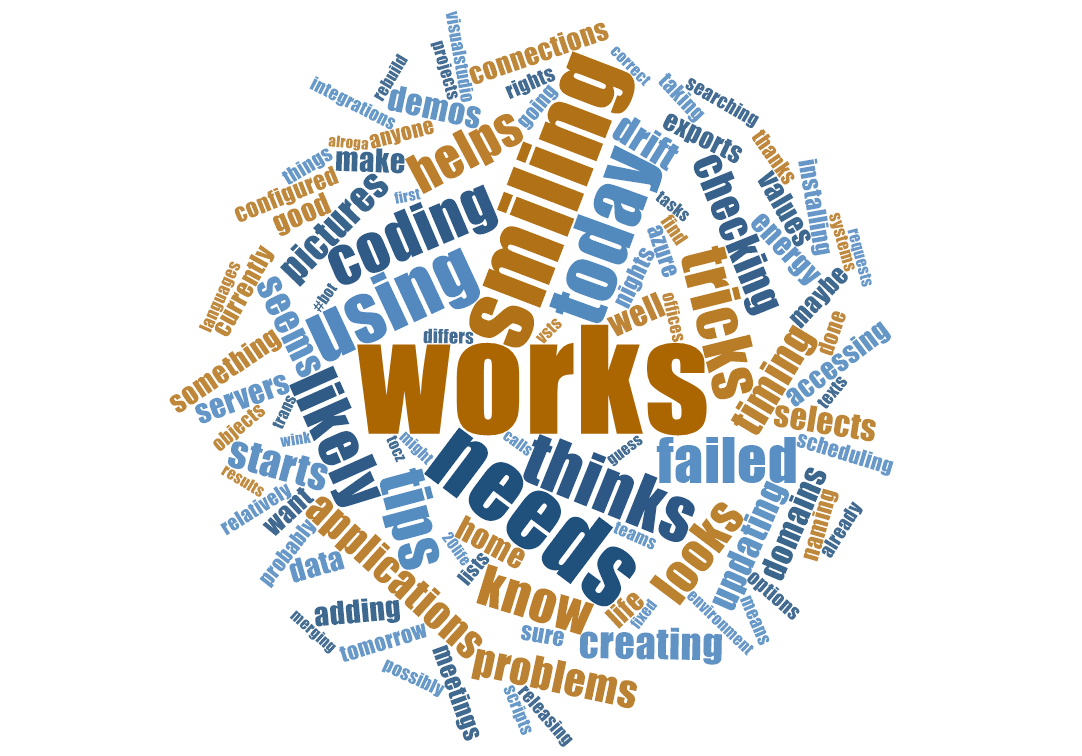
\includegraphics[width=1.05\textwidth]{wordcloud.png}
\caption{Word cloud of the first 100 most used words.}\label{fig:wordcloud}
\index{figures}
\end{figure}



\begin{table}
\centering
\caption{The most frequent words} \label{table:word}
\begin{tabular}{cc}
\hline
\textbf{Word} & \textbf{Count} \\ \hline
Works & 2770 \\
Smiling & 1900 \\
Changing & 1216 \\
Needs & 1186 \\
Deploys & 1154 \\
Tricks & 1130 \\
Tips & 1125 \\
Today & 971 \\
Thinks & 916 \\
Issues & 833 \\
\hline
\end{tabular}
\end{table}


 We also did an automatic sentiment analysis of help, general, and backend channels and found the results that are presented in Table \ref{table:sentiment}. Generally, tone of the voices is more neutral, but in the help channel there are more mixed, negative and positive sentiments found compared to the other channels.
 
\begin{table}
\centering
\caption{Sentiment analysis results} \label{table:sentiment}
\begin{tabular}{lc}
\hline
\textbf{Codes} & \textbf{n} \\ \hline
Operations - Mixed&0\\
Operations - Negative&6\\
Operations - Neutral&292\\
Operations - Positive&1\\ \hline
General - Mixed&2 \\
General - Negative&6 \\
General - Neutral&43 \\
General - Positive&8 \\ \hline
Help - Mixed&107\\
Help - Negative&62\\
Help - Neutral&354\\
Help - Positive&32 \\ \hline
Backend - Mixed&4\\
Backend - Negative&8\\
Backend - Neutral&79\\
Backend - Positive&11\\
\hline
\end{tabular}
\end{table}

Also, after coding the logs from three weeks of conversations in general, backend, and operations channels we came to the results presented in Table \ref{table:coded}.

\begin{table}
\centering
\caption{Number of conversation coded in each category in three channels} \label{table:coded}
\begin{tabular}{lccc}
\hline
 & \textbf{Backend} & \textbf{General} & \textbf{Operation} \\ \hline
\textbf{General Answer}&50 &50 &10 \\
\textbf{General Informing}&20 &5 &45 \\
\textbf{General Question}&15 &10 &15 \\
\textbf{Technical Answer}&110 &130 &100 \\
\textbf{Technical Informing}&170 &25 & 150\\
\textbf{Technical Question}&125 &60 &115 \\
\textbf{Socializing}&5 &15 &4 \\
\textbf{Emoji}&15 &90 &70 \\
\hline
\end{tabular}
\end{table}

Here in Table \ref{table:coded} we have the number of codes for each category and see that for example the usage of emoji in the general channel is 6 times more than the backend channel. Respectively number of technical questions drops dramatically in the general channel compared to both backend and operations channel. General questions are asked almost the same in all three channels.

We also looked at number of messages sent per hour in backend and frontend channels. Early in the morning, between 8:00 and 9:00 is the busiest time, in which 686 messages are sent. Then between 9:00 and 13:00 the number of messages sent are stable at around 500 messages per hour, and then halves until 14:00. Then suddenly the number of messages drops substantially to around 90 at 15:00 and steadily goes down until 5:00 in the morning that again starts to rise.

\begin{figure}[hbt!]
\centering
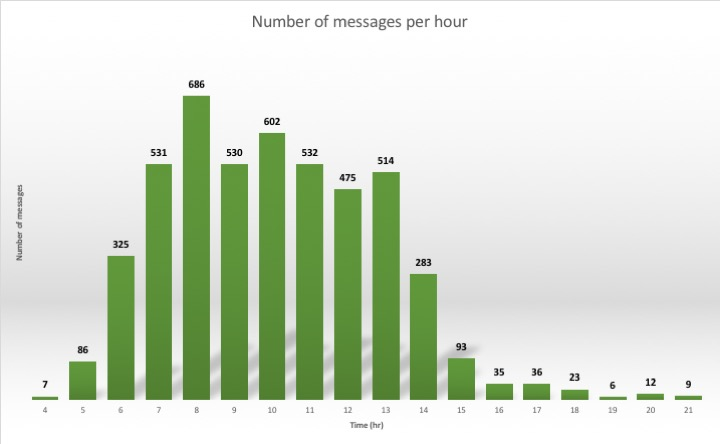
\includegraphics[width=.99\textwidth]{be-fe-messageperhour.jpg}
\caption{Number of messages sent per hour in backend and frontend channels}\label{fig:mph}
\index{figures}
\end{figure}

At the same channels, i.e. backend and frontend, we also looked at the user activity. For privacy reasons the usernames are not converted to real names. Here we see that there are three users who have sent around 500 messages, four other users have also sent more than 200 messages. In total there are 11 users out of 38 who have sent more than 100 messages. 

\begin{figure}[hbt!]
\centering
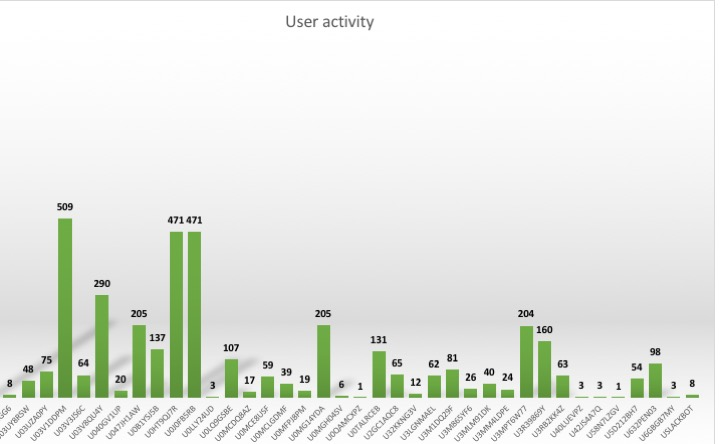
\includegraphics[width=.99\textwidth]{be-fe-useractivity.jpg}
\caption{User activity in backend and frontend channels}\label{fig:useractivity}
\index{figures}
\end{figure}



%\pagebreak
\clearpage
%%%%%%%%%%%%%%%%%%%%%%%%%%%%%%%%%%%%%%%%%%%%%%%%%%%%%%%%%%%%%%%
\section{The survey}
%%%%%%%%%%%%%%%%%%%%%%%%%%%%%%%%%%%%%%%%%%%%%%%%%%%%%%%%%%%%%%%

A total of 112 responses were gathered, of which 95 were completed to the extent that was usable and analyzable. Out of 95 respondents, 87 percent were male (n = 83), and 13 percent female (n = 12) with a mean age of 32 years old (n = 95). Percentage of the respondents who reported that they were working in team was 96 (n = 91), and the proportion of people working in co-located teams (n = 46, 48\%) were slightly less than those who reported working in distributed teams (n = 49, 52\%). The proportion of the team size among the respondents was one-third being in teams of two to five members, one-third in teams with six to eight members and one-third in teams with nine or more members. Table \ref{table:ds} shows the descriptive statistics. 


Among all the respondents, 69\% were software developers, and the rest had roles such as designer, software architect, and manager (Table \ref{table:roles}). The respondents were also asked whether they consider themselves front-end developer, back-end developer or other types of developers. 36\% of all respondents considered themselves as other type of the developers, 26\% considered themselves as back-end developers and 7\% as front-end developers (Table \ref{table:roledetail}). Here there is no meaningful difference between the results gathered through Reddit vs. snowball sampling, except that there were 10\% more back-end developers responding to the survey compared to Reddit users. Looking at the other roles we see that none of the respondents considered themselves as pure testers, which was somehow expected, since the survey was posted in developers forums. 

\begin{figure}[hbt!]
\centering
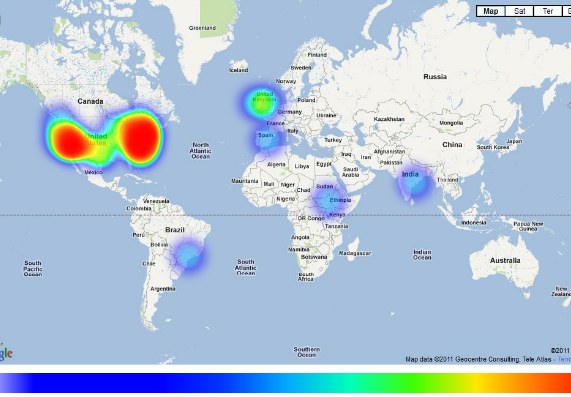
\includegraphics[width=.99\textwidth]{heatmap.png}
\caption{A heatmap of the respondents location}\label{fig:heatmap}
\index{figures}
\end{figure}


\begin{table}
\centering
\caption{Descriptive statistics} \label{table:ds}
\begin{tabular}{lllcc}
\hline
 & \textbf{Unit} & \textbf{n} & \textbf{Mean(M)} & \textbf{Median} \\ \hline
\textbf{Meetings} & Frequency per day & 63 & 2.9 & 3 \\
\textbf{Time in meetings} & Hours per day; \ac{dsm}s included & 48 & 1.4 & 1 \\
\textbf{Team size} & Members including self & 87 & 8.1 & 7 \\
\hline
\end{tabular}
\end{table}



\begin{table}
\centering
\caption{Respondents roles in teams} \label{table:roles}
\begin{tabular}{lcc}
\hline
 & \textbf{n} & \textbf{\%} \\ \hline
\textbf{Developer}&66&69\\
\textbf{Tester}&2&2\\
\textbf{Software Architect}&7&7\\
\textbf{Designer}&9&10\\
\textbf{Manager}&2&2\\
\textbf{Other}&9&10\\
Total&95&100\\
\hline
\end{tabular}
\end{table}


\begin{table}
\centering
\caption{Respondent’s roles in detail} \label{table:roledetail}
\begin{tabular}{lllcc}
\hline
 & \textbf{n(Total)} & \textbf{\%(Total)} & \textbf{\%Reddit} & \textbf{\%Snowballing} \\ \hline
\textbf{Front End Developer}&7&7&8&6 \\
\textbf{Back End Developer}&25&26&23&33 \\
\textbf{Developer}&34&36&35&37 \\
\textbf{Tester}&2&2&0&6 \\
\textbf{Software Architect}&7&7&8&6 \\
\textbf{Designer}&9&10&13&3 \\
\textbf{Manager}&2&2&2&3 \\
\textbf{Other}&9&10&11&6 \\
Total&95&100&100&100 \\
\hline
\end{tabular}
\end{table}

Scrum was the most used development method among the respondents, with almost half of the respondents using it, followed by Kanban which is reported to be used by a quarter of the respondents (Table \ref{table:dm}). The most popular communication media in teams, according to the respondents, were instant messaging (\ac{im}). It is used by more than 90 percent of the respondents. Email follows closely the \ac{im} and is reported to be used by almost 80 percent of the respondents. Face-to-face meetings is the least used communication media by teams, and just 17 percent of our respondents use it (Figure \ref{fig:com-media}).

\begin{table}
\centering
\caption{Development methods used in teams} \label{table:dm}
\begin{tabular}{lcc}
\hline
 & \textbf{n} & \textbf{\%} \\ \hline
\textbf{Scrum}&31&47\\
\textbf{Kanban}&16&24\\
\textbf{Scrumban}&8&12\\
\textbf{XP}&5&8\\
\textbf{Waterfall}&6&9\\
Total&66&100\\
\hline
\end{tabular}
\end{table}



\begin{figure}[hbt!]
\centering
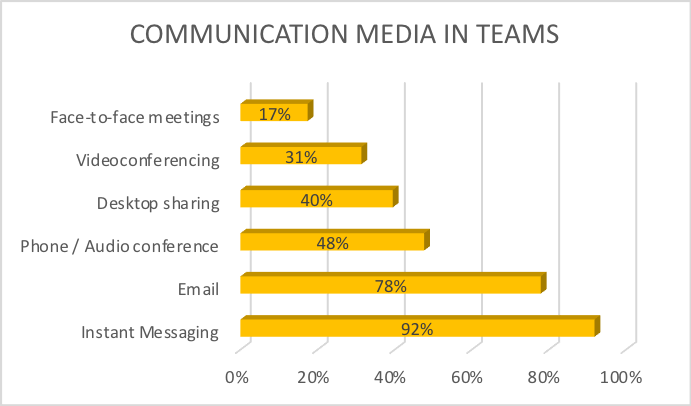
\includegraphics[width=.99\textwidth]{media-in-teams.png}
\caption{Communication media used in teams}\label{fig:com-media}
\index{figures}
\end{figure}



When focusing on specific communication tools, we see that Slack is the biggest winner here, with 59 percent of the respondents using it as their number one means of communication with other team members (Figure \ref{fig:com-tools}). Skype follows Slack by a good distance, and only 38 percent of the respondents use as a communication tool. The third place is occupied by Google Hangout. It is worth mentioning here that Skype and Hangout are more famous for their video calling abilities, while Slack is more text-based, so there would be difficult to compare these tools with each other. In this list Webex, Google Hangout and Skype can be grouped with each other and Slack, HipChat and MS-Teams can be compared to each other (Figure \ref{fig:com-tools}).


\begin{figure}[hbt!]
\centering
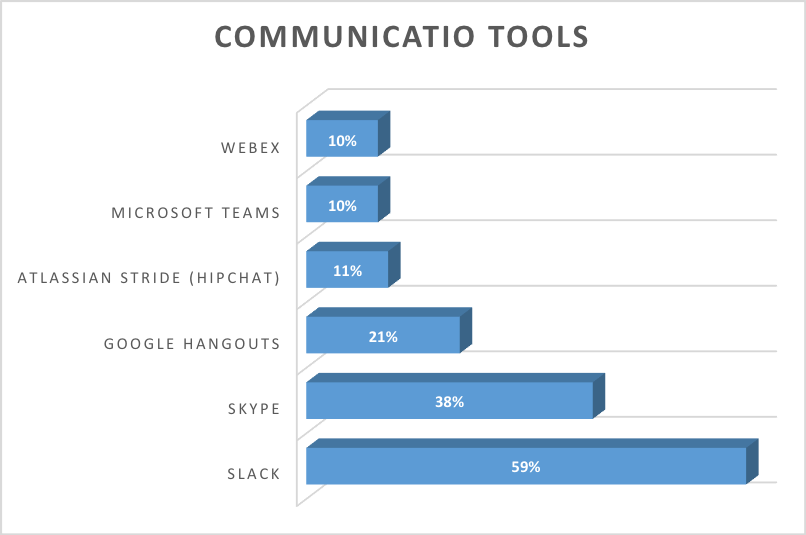
\includegraphics[width=.99\textwidth]{com-tools.png}
\caption{Communication tools used in teams}\label{fig:com-tools}
\index{figures}
\end{figure}

The respondents were also asked what was their biggest challenge while working distributed and almost half of them chose time-zone difference as their biggest challenge. There is no surprise that coordination comes as the second challenge, being chosen by 43 percent of the respondents. Being in different time-zones will immediately affect the coordination between team members. Also, one-third of the respondents chose communication and trust as one of their challenges in their distributed teams (Figure \ref{fig:challenges}).

\begin{figure}[hbt!]
\centering
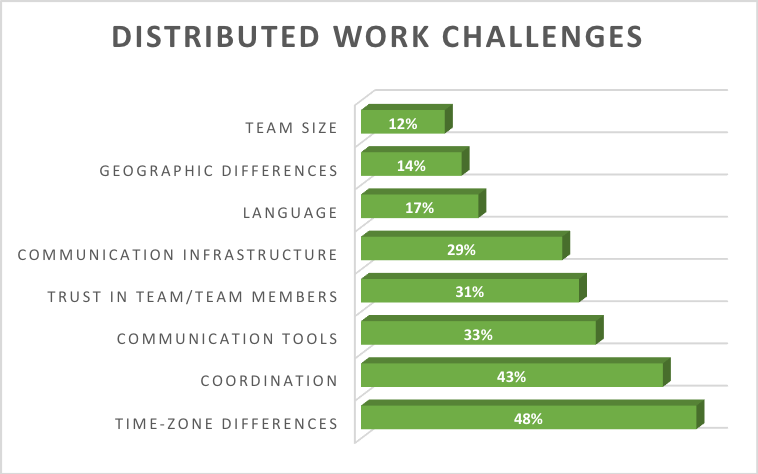
\includegraphics[width=.99\textwidth]{challenges.png}
\caption{Challenges often confronted in distributed teams}\label{fig:challenges}
\index{figures}
\end{figure}

When asked about the frequency of their face-to-face and in-person meetings, one-third of the respondents reported that they never met other team members. 20 percent reported meeting every month, and about one-third chose “other” as the answer to the question (Table \ref{table:f2f}). I also asked the respondents about the purpose of such meetings, and the prominent answer was “status update”, chosen by 27 percent of the respondents. Information sharing and brainstorming were ranked as the second and third purpose of the meetings, chosen respectively by 21 and 15 percent of the respondents (Figure \ref{fig:purpose}). 

\begin{table}
\centering
\caption{Frequency of face-to-face team meetings} \label{table:f2f}
\begin{tabular}{lcc}
\hline
 & \textbf{n} & \textbf{\%} \\ \hline
\textbf{Never}&15&34\\
\textbf{At project kick-off only}&0&0\\
\textbf{Monthly}&9&20\\
\textbf{Every 6 months}&5&11\\
\textbf{Yearly}&2&5\\ 
\textbf{Other}&13&30\\ 
Total&44&100\\
\hline
\end{tabular}
\end{table}


\begin{figure}[hbt!]
\centering
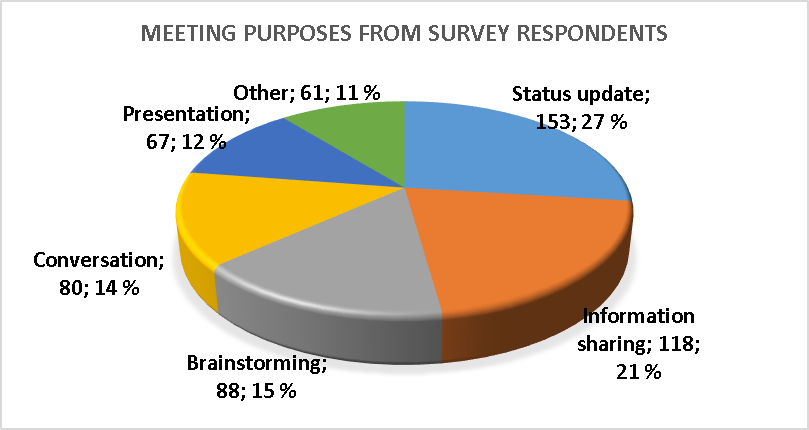
\includegraphics[width=.99\textwidth]{purpose.png}
\caption{Purposes of team meetings}\label{fig:purpose}
\index{figures}
\end{figure}
%\chapter{Discussion}

In this chapter, the results presented in chapter four, including their limitations are discussed about the related research and theories. In the beginning, the results of the case study will be discussed followed by the results of the survey.

To verify that the results of our survey are a good representative of the active programmers we decided to compare our results with the Stack Overflow’s 2018 developer survey results\footnote{\url{https://insights.stackoverflow.com/survey/2018/}}. Stack Overflow is a question and answer forum dedicated to computer programming and every year runs a survey among its users and shares it openly with the community. This year more than 100,000 developers participated in the survey, and its results were published shortly after our survey and could be considered as a good reference. 
Looking at the heat map of the location of the subjects, we see that there are similarities between the two surveys. Most of the respondents are from northern America, Europe, and India. Regarding gender, there were slightly more female participants in our study. There were almost double as much backend developers in Stack Overflow’s survey than ours. 

\citet{Stray2017a} also did a survey of distributed teams and found almost identical demographic results as our survey, which combined with the Stack Overflow results ensures us that our results are reliable. 
However, when it comes to time spent on active remote collaboration; there is a slight difference between our findings with \citet{Karis2016} who ran a survey among Google developers. Out of 501 responses they received, 6.6 percent stated that they were collaborating nearly all the time while in our case (n = 44), nobody was claiming to collaborate that much. Table \ref{table:collaboration} compares the results.
    
    
\begin{table}
\centering
\caption{Time spent on active remote collaboration} \label{table:collaboration}
\begin{tabular}{lcc}
\hline
\textbf{The frequency of active collaboration} & \textbf{Our results} & \textbf{Google} \\ \hline
None or nearly none of my time&11\%&10.8\%\\
Less than 1/4 of my time&64\%&53.1\%\\
Up to 1/2 of my time&20\%&22.8\%\\
More than half my time&5\%&6.8\%\\
Nearly all my time&0\%&6.6\%\\
&Total n=44&Total n=501\\
\hline
\end{tabular}
\end{table}

If we consider a typical workweek as forty hours, then this amount of remote collaboration counts as around 14\% of the whole people engaged in distributed teams spending at least 21 hours per week in active collaboration with distributed team members. Also, 24\% spend some time between 10 to 20 hours a week on remote collaboration. 

These numbers become even more meaningful if we look at the responses we have got about the challenges in the distributed work, where around half of the respondents have stated that time-zone differences and coordination are the biggest challenges in distributed work. 
If the task or the project that the team members are working on can be divided into parts that can partly be done and worked on individually and independent from other team members then it would be easier to collaborate remotely with other team members, since the time needed to work on a given task simultaneously is minimal or non-existent. 

The problem arises when two team members must work on the same task remotely; then it could be a huge challenge if the time difference is so much that at one place the sun is shining at the middle of the day while in the other part of the world it has past a few hours after midnight. 
Here there is a dilemma between having a development team that can work around the clock, 24 hours a day or a development team that are far less separated, both physically and by time. The choice might be dependent on kind of the project and tasks, but our research shows that there would be unexpected challenges in coordination and collaboration between team members that can affect the results gained by distributed team heavily. 

Finding of \citet{Ibrahim2015} also shows that temporal and geographical distance is the biggest challenge of distributed software development. More than 75 percent of the literature reported it as the number one challenge among the distributed teams. Distance differences also affect communication negatively in teams; it reduces the efficiency of communication between remote teams \citep{Dorairaj2011}.

\citet{Marlow2016} in their survey asked a question about the purpose of remote meetings. We did the same and Table \ref{table:remotepurpose} compares the results. According to the results of our survey, almost half of the respondents reported use scrum as their development method. So it is considered that the most stated reason for remote meetings is “status update.” “Information sharing” follows closely status update, while the status update is obviously about updating the whole team, information sharing might refer to meeting and collaboration with two team members.

\begin{table}
\centering
\caption{The purpose of remote meetings} \label{table:remotepurpose}
\begin{tabular}{lcc}
\hline
& \textbf{Our results} & \textbf{Marlow 2016} \\ \hline
Status update&27\%&33\%\\
Information sharing&21\%&18\%\\
Brainstorming&	15\%&	13\%\\
Conversation&	14\%&	12\%\\
Presentation&	12\%&	9\%\\
Other&	11\%&	14\%\\
\hline
\end{tabular}
\end{table}

Looking at the communication media used in distributed teams we see that just 17\% have stated that they use face-to-face meetings as a communication media, and later in another question when asked about the frequency of face-to-face meetings we see that 34\% of respondents have stated that they never meet face-to-face with other team members. This can be problematic and increases misunderstanding among the team \citep{Curtis1988}.


\chapter{Limitations}






\printbibliography[heading=bibintoc]
%\nocite{Nyrud2017a} %For referring to references not used in the article!!!

%\appendix
%\chapter{Survey Questions}
%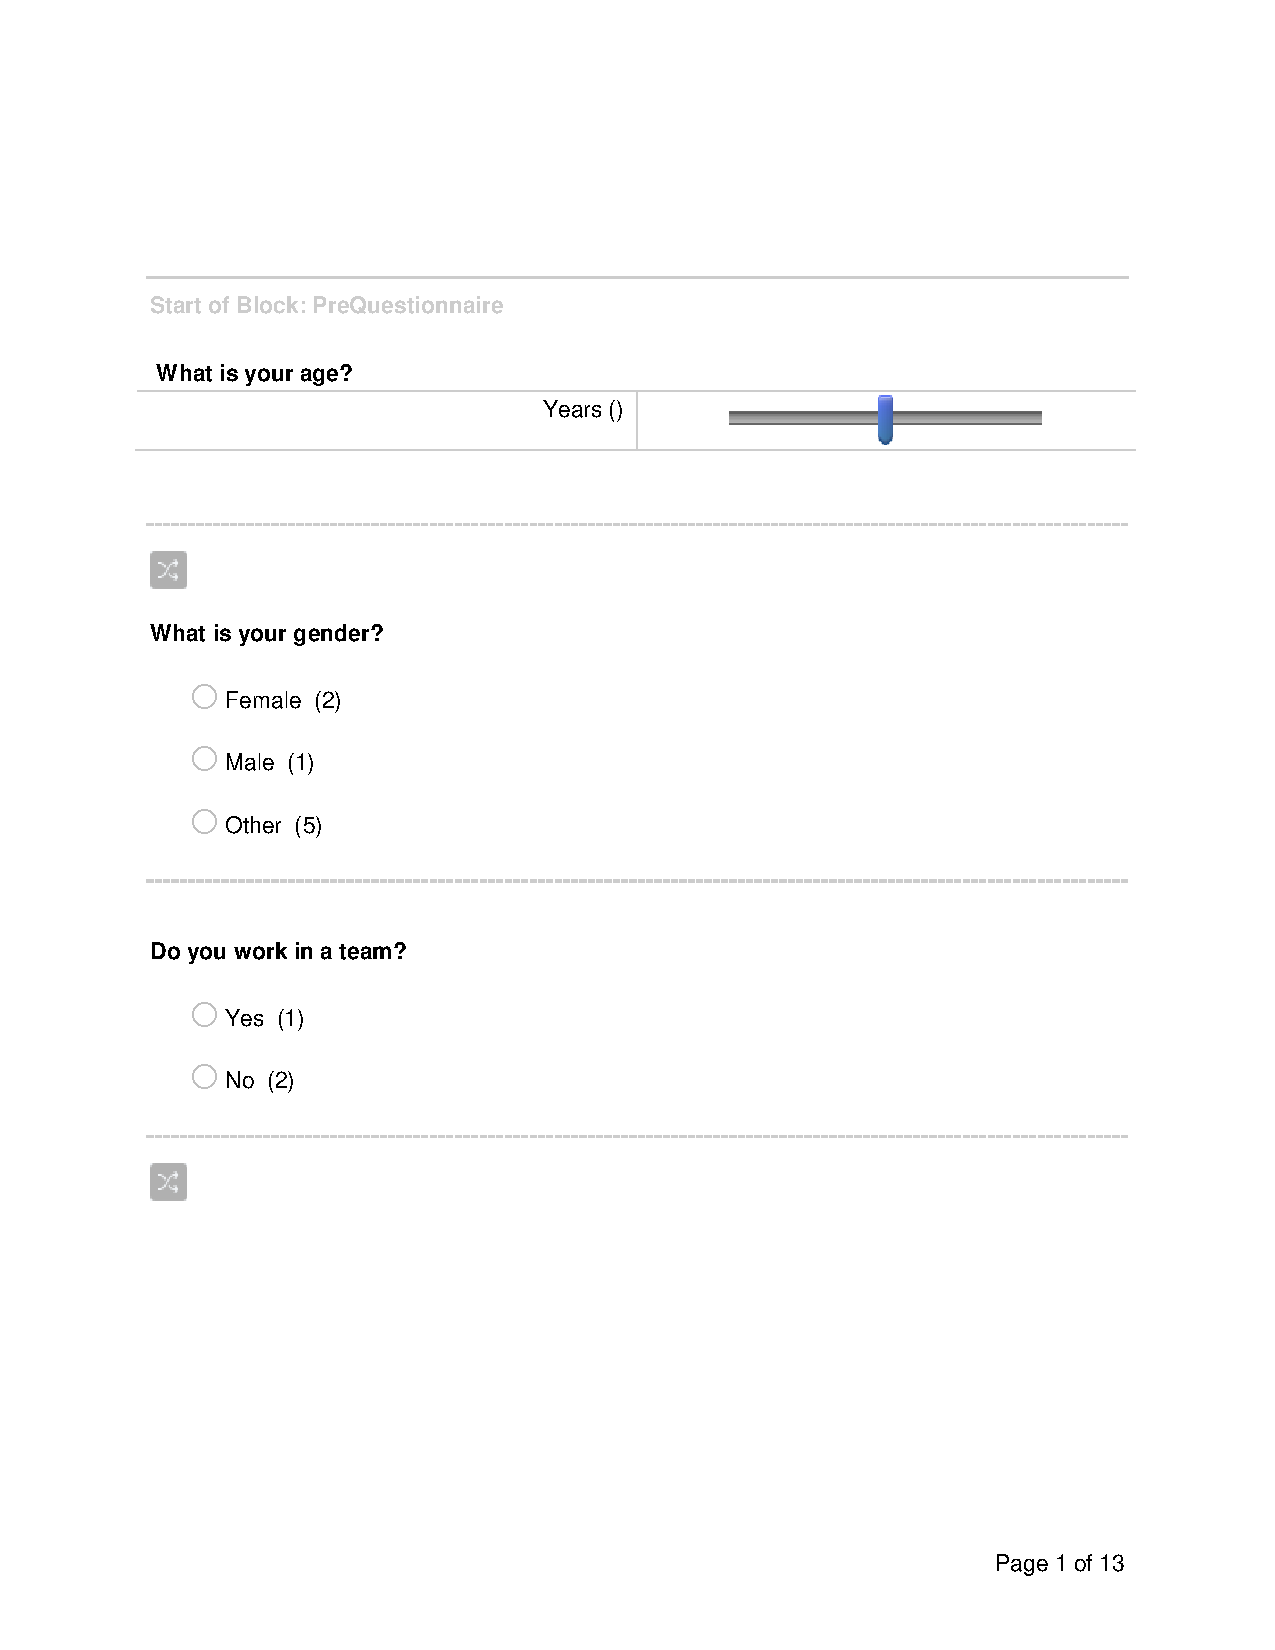
\includepdf[pages=-, scale=0.9, pagecommand={}]{survey.pdf} 


%\printindex
%\theendnotes
%% Pocket materials at the VERY END of thesis
%\pocketmaterial
%\extrachapter{Pocket Material: Map of Case Study Solar Systems} 
\end{document}